% =====================================================================
% Determinacy-Field Mechanics -- arXiv draft (v0.3, 2026-07-20)
% Written per docs/HANDOFF_PAPER_V2.md (sole authoritative writing brief).
% v0.2: all 21 adjudicated items of the fifth AI mock review applied
%       (claim-level restriction, axiom clarifications A2/A5/A10,
%       E6' pair-update transcription, benchmark-input fixing,
%       reproducibility metadata; adjudication record: docs/DERIVATIONS.md
%       Sec. 16).
% v0.3: English proofreading pass. Three external AI proofreading
%       reports (ChatGPT / Grok / Gemini, 2026-07-20) adjudicated and
%       applied: grammar, idiom, compound-modifier consistency
%       (clock-and-light sector), jargon reduction, and precise wording
%       for the V6 gate factor and the V16 reference clock (both fixed
%       against the implementation). No number, claim, equation, or
%       mandated positioning phrase changed.
% Input canon: docs/DERIVATIONS.md, docs/PHYSICS.md v1.6,
%              docs/THEORY_SYNTHESIS.md v1.7, index.html v1.23.
% Target: American Journal of Physics / European Journal of Physics
%         (arXiv: physics.ed-ph primary, gr-qc cross-list).
% Build:  pdflatex dfm-paper.tex  (RevTeX 4.2; see paper/README.md)
% =====================================================================
\documentclass[aps,reprint,amsmath,amssymb,nofootinbib,superscriptaddress,floatfix]{revtex4-2}

\usepackage{graphicx}
\graphicspath{{figures/}}
\usepackage{bm}
\usepackage{hyperref}

\newcommand{\ud}{\mathrm{d}}
\newcommand{\vect}[1]{\bm{#1}}
\newcommand{\Kt}{K_t}
\newcommand{\Dz}{D_0}

\begin{document}

\title{Determinacy-Field Mechanics: A Machian Toy Universe with Tunable
Frame Dragging, Emergent Inverse-Square Gravity, and Spin-as-Heat
Thermodynamics}

\author{Tetsuya Imamura}
% Affiliation confirmed 2026-07-18 (author's decision).
\affiliation{Independent Researcher, Tokyo, Japan}

\date{July 20, 2026}

\begin{abstract}
We present Determinacy-Field Mechanics (DFM), an educational toy model in
which a single scalar field $W$ (the ``determinacy field,'' sourced by
point masses as $w = m/\sqrt{d^2+\varepsilon^2}$) simultaneously plays
four roles---the weight defining the local inertial frame, the
gravitational potential, the local clock rate, and the optical
refractive index---while a single signed spin degree of freedom $s$ per
particle acts as heat.
The model is specified by axioms A1--A13 and update rules E1$'$--E11 on a
two-dimensional Euclidean background, and is implemented as a
self-contained single-file HTML simulator whose principal claims are
machine-verified by an embedded test suite.
A one-parameter background determinacy $\Dz$ interpolates continuously
between Newtonian absolute space ($\Dz \to \infty$) and a fully
relational, Machian space ($\Dz \to 0$), turning Newton's bucket into
an executable parameter scan.
With frame dragging amplified to order unity ($k_F = 1$), disk systems
develop a modest outer-velocity enhancement---a machine-gated increase
in the outer rotation velocities relative to the $k_F = 0$ control---as
a demonstration of the mechanism within the model; with $k_F = 0$ the
dynamics reduces exactly to Newtonian $N$-body gravity.
Under the single calibration $\Kt = c^2/G$, and with the observational
inputs for each benchmark specified in an appendix, the model's
weak-field clock-and-light sector reproduces the leading weak-field
benchmark formulas for the GPS clock offset, the solar-limb light
deflection, and
the Shapiro delay (formula-level benchmark agreement), with the
gravitational-to-optical ratio $1{:}2$ fixed by the single axiomatic
exponent choice $a = b = 1$ rather than by per-observable fitting; the
same dynamics does \emph{not} reproduce the static first
post-Newtonian perihelion advance of Mercury, and we exhibit this
failure in the same calibration table.
We state explicitly what the model does not claim: it is not a
description of the real universe; it does not remove the need for dark
matter; it has neither Lorentz invariance nor causal propagation; and
its thermodynamic sector is an analogy rather than a quantitative
theory.
DFM is offered as a compact, fully inspectable laboratory for teaching
and exploring Machian ideas, weak-field phenomenology, and conservation
bookkeeping in interactive form.
\end{abstract}

\maketitle

% =====================================================================
\section{Introduction}
\label{sec:intro}

Newton's rotating bucket poses one of the oldest questions about
inertia: with
respect to \emph{what} does the water's surface curve?~\cite{Newton1687}
Newton answered ``absolute space''; Mach countered that only the
relative configuration and motion of matter can matter, so the distant
stars themselves must define the inertial standard~\cite{Mach1883}.
Sciama later sketched how inertia could be induced by distant
matter~\cite{Sciama1953}, and Barbour and Bertotti gave relational
mechanics a rigorous variational formulation~\cite{BarbourBertotti1982}.
In the real universe, general relativity (GR) settles the question in a
subtle way: matter does drag local inertial frames (the Lense--Thirring
effect~\cite{LenseThirring1918}), but the effect is suppressed by
$v/c^2$ factors and is minute---milliarcseconds per year for Earth
satellites, confirmed by Gravity Probe~B and LAGEOS
ranging~\cite{Everitt2011,CiufoliniPavlis2004}.

This paper asks a deliberately counterfactual question and builds the
smallest working model that answers it:
\emph{what would mechanics look like if frame dragging were an
order-unity effect?}
The model we construct in response, Determinacy-Field Mechanics (DFM),
is
\emph{a Machian toy model on a fixed Euclidean background that makes the
inertial standard emergent from the matter distribution}.
Every point mass $j$ contributes a scalar ``determinacy''
$w_j = m_j/\sqrt{d_j^2+\varepsilon^2}$ ($\to m_j/d_j$ as
$\varepsilon \to 0$), quantifying how strongly it pins down the spatial
coordinates near it.
The total field $W = \Dz + \sum_j w_j$, together with one signed spin
scalar $s_i$ per particle, then plays every dynamical role in the model:
the determinacy-weighted average of the sources' motion defines the
local frame $\vect{u}(\vect{r})$ against which inertia holds; the
gradient of $W$ is the gravitational acceleration; a single
dimensionless potential $\psi = W/\Kt$ sets both the local clock rate
and the optical refractive index; and spin doubles as heat, generating
pressure through spin-induced frame rotation.

The model is intentionally not a candidate description of nature.
It is an educational and exploratory instrument in the tradition of
toy universes: small enough to specify completely in a few pages
(axioms A1--A13, update rules E1$'$--E11, consequences T1--T9),
concrete enough to run as a self-contained single-file HTML application
with no external dependencies, and honest enough that every quantitative
claim made below is checked by machine-verifiable tests embedded in the
implementation (\texttt{HP.verify.all()}, fourteen checks, plus a
107-item continuous-integration suite).
Where a claim holds only for particular initial conditions or parameter
ranges, we say so and label it a \emph{conditional numerical
proposition} rather than a theorem.

\subsection{Contributions}
\label{sec:contributions}

The paper's contributions, stated with their intended scope:

\begin{enumerate}
\item[C1.]{\bf Minimality and implementability.}
A system of thirteen axioms and eleven update rules (A1--A13,
E1$'$--E11) is shown to be consistent within the verified parameter
range and to
run as a single-file numerical implementation---an existence proof by
implementation.

\item[C2.]{\bf Structural decomposition of Newtonian gravity.}
Taking the gradient of the determinacy $w \propto m/d$ as the
acceleration (axioms A3 and A6) yields the inverse-square law, since
$\nabla(m/d) \propto m/d^2$.
This is \emph{not} a derivation of gravity from nothing; it is a
decomposition of the gravitational law into two assumptions---the field
distance law $w \propto m/d$ and the gradient response
$\vect{a} = G\nabla W$.
We note that on a two-dimensional plane a Gauss-law-consistent field
would instead fall off as $1/d$; DFM deliberately posits the
three-dimensional-like distance law on the plane (a pseudo-3D
idealization, Sec.~\ref{sec:axioms}).

\item[C3.]{\bf Structural correspondence with weak-field GR.}
Under the parameter mapping $\Kt = c^2/G$, the model's proper-time and
light-deflection formulas have the same structure as weak-field GR
(Sec.~\ref{sec:corr}).
Beginning with version 1.7 of the model, clock rate and refraction are
generated
by the single potential $\psi$ through $N = e^{-a\psi}$ and
$A = e^{+b\psi}$ with the exponents fixed once, axiomatically, at
$a = b = 1$; under that choice the effective lensing coefficient is the
derived combination $(a+b)/\Kt = 2/\Kt$ and is never retuned per
observable.

\item[C4.]{\bf Continuous interpolation between absolute and relational
space.}
The background determinacy $\Dz$ connects Newtonian absolute space
($\Dz \to \infty$) to a fully relational space ($\Dz \to 0$) with one
dial, converting Newton's bucket argument into an executable parameter
scan.

\item[C5.]{\bf Mechanism demonstration of outer-velocity enhancement.}
With dragging amplified to $k_F = 1$, disk systems exhibit higher
outer rotation velocities relative to the $k_F = 0$ Keplerian control
run from identical initial conditions (machine-gated gain
$0.055 \pm 0.007$; outer-band ratio $1.082$ at 6000 steps).
This demonstrates \emph{mechanism sufficiency for outer-velocity
enhancement within the model}---not flatness of the curve
(Sec.~\ref{sec:exp2})---and is not a claim about real galaxies
(Sec.~\ref{sec:negative}).

\item[C6.]{\bf Emergent thermodynamic behavior from spin-as-heat.}
Contact friction converting translation to spin, spin diffusion, and
spin repulsion together produce temperature equilibration (a
zeroth-law analogue) and pressure.

\item[C7.]{\bf Exact conservation laws.}
The reciprocity axiom A13 with the revised rules E5$'$/E6$'$/E10$'$
makes linear momentum and total angular momentum (orbital $+$ spin)
exactly conserved \emph{at the equation level} (T7, proved pairwise in
Sec.~\ref{sec:dynamics}); the finite-step numerical residual of the
verification run is at the single-precision rounding floor and is
independent of the time step (Table~\ref{tab:verify}).
The reaction bookkeeping further yields outward angular-momentum
transport, spin--orbit synchronization, and tidal-migration analogues.

\item[C8.]{\bf Derivation and delimitation of the dragging precession.}
For prograde orbits around a prograde-spinning center, E6$'$ makes the
periapsis \emph{regress} (machine check V6), with leading scaling
$\Delta\varpi/\mathrm{orbit} \propto -k_F S_c R_c^2/\sqrt{GMa}$.
The sign and the spin$\times$radius$^2$ ($\propto J$) factor agree with
the GR Lense--Thirring periapsis precession, but the radial power
differs in the near zone ($a^{-1/2}$ per orbit versus $a^{-3/2}$ for
Lense--Thirring), and the static first post-Newtonian (1PN) perihelion
advance is not reproduced (Sec.~\ref{sec:negative}).
The model also exhibits a background-crossover scale
$r_{\rm bg} \sim M_d/\Dz$ beyond which the background determinacy
screens the disk's frame contribution---an estimate of where the
outer-velocity enhancement must die away, not a prediction of a flat
segment (Sec.~\ref{sec:exp2}).
\end{enumerate}

\subsection{What this paper does not claim}
\label{sec:nc-summary}

Because the credibility of a toy-model paper rests on the absence of
overclaiming, we summarize here the negative claims that
Sec.~\ref{sec:negative} states in full:
(1)~DFM is not proposed as a description of the real universe;
(2)~the outer-velocity-enhancement demonstration does not imply that
dark matter is unnecessary;
(3)~the model has no Lorentz invariance and no causal (finite-speed)
propagation of the field;
(4)~it is two-dimensional and makes no 3D quantitative predictions;
(5)~it does not reproduce the static 1PN perihelion advance of Mercury;
and
(6)~its thermodynamic sector is a qualitative analogy, not a
quantitative thermodynamic theory.

\subsection{Relation to prior work}
\label{sec:prior}

DFM deliberately draws on several bodies of literature without
belonging fully to any one of them.
Sciama's inertial-induction proposal~\cite{Sciama1953} is the closest
ancestor in spirit; DFM differs by being an explicit, executable
discrete dynamics rather than a field-theoretic sketch.
Barbour--Bertotti relational mechanics~\cite{BarbourBertotti1982}
derives from a variational principle; DFM currently lacks an action
principle (open problem L1, Sec.~\ref{sec:limits}) and should be read
as a phenomenological simplification.
The flat-rotation-curve literature---the observations~\cite{RubinFord1970},
the dark-matter interpretation constrained by CMB and lensing
statistics~\cite{Planck2018}, and MOND~\cite{Milgrom1983}---is
relevant here only as context for a third class of mechanisms
(dragging amplification) demonstrated within the model.
Claims that GR gravitomagnetism alone explains flat rotation curves
have been made~\cite{CooperstockTieu2005,Ludwig2021} and challenged
by subsequent analyses concerning the source model, singular matter
layers, and the magnitude of the gravitomagnetic
contribution~\cite{FuchsPhleps2006,Korzynski2007,LasenbyHobsonBarker2023};
DFM does not enter that controversy, because it makes $k_F$ a free
dial and studies the counterfactual.
Relational reformulations of classical mechanics itself have a
continuing literature beyond Barbour--Bertotti: Lynden-Bell and Katz
showed that mechanics without absolute space is equivalent to Newtonian
mechanics in a zero-angular-momentum universe~\cite{LyndenBellKatz1995},
and Assis has developed a Weber-force implementation of Mach's
principle~\cite{Assis1999}; DFM shares their motivation but trades
variational rigor for an executable field construction.
The optical-medium formulation of light in a gravitational field goes
back to classic work~\cite{deFelice1971}; our light rule E8R is a
direct descendant with the medium additionally \emph{advected} by the
frame field.
Light carried by a moving medium is also the defining structure of
acoustic and analogue gravity---Unruh's sonic horizon~\cite{Unruh1981}
and the analogue-gravity programme reviewed by Barcel\'o, Liberati, and
Visser~\cite{BarceloLiberatiVisser2005}---of which E8R is a simple
member (an effective acoustic-type geometry with flow field $\vect{u}$),
although DFM makes no horizon-thermodynamics claims.
The attitude that gravity and inertia may be emergent
phenomena~\cite{Verlinde2017} is shared, but no thermodynamic or
holographic derivation is attempted.
Finally, the spin-as-heat sector is a cousin of granular-gas kinetic
theory~\cite{BrilliantovPoschel2004} with a non-local spin repulsion
that has no counterpart there.

\subsection{Outline}

Section~\ref{sec:axioms} states the axioms, Sec.~\ref{sec:dynamics} the
update rules.
Section~\ref{sec:corr} gives the Newtonian reduction, the weak-field GR
mapping with its real-data calibration (including the Mercury failure),
and the structural differences.
Section~\ref{sec:experiments} presents six numerical experiments with
machine-verified results.
Section~\ref{sec:negative} states the limitations and negative claims,
and Sec.~\ref{sec:conclusion} outlines future work.
Appendix~\ref{app:si} restores SI units,
Appendix~\ref{app:inputs} fixes the benchmark inputs and verification
configurations, and Appendix~\ref{app:theorems} tabulates the
consequences T1--T9 with their conditions and machine gates.

% =====================================================================
\section{Axioms}
\label{sec:axioms}

\subsection{Ontology and notation}

The world consists of a finite set of point particles indexed by $i$,
with mass
$m_i$, position $\vect{r}_i$, velocity $\vect{v}_i$, and a signed spin
scalar $s_i$ (angular velocity about the out-of-plane axis), evolving
in discrete time on a two-dimensional Euclidean plane.
Particles have a finite disk radius $R_i = r_R\sqrt{m_i}$ and moment of
inertia $I_i = \tfrac{1}{2}m_iR_i^2$.
We write $d_j = |\vect{r}-\vect{r}_j|$,
$\hat{n}_{ij} = (\vect{r}_i-\vect{r}_j)/d_{ij}$, and
$\hat{z}\times(x,y) = (-y,x)$.
The softening length $\varepsilon$ is a numerical regularization, not
part of the theory (Sec.~\ref{sec:dynamics}).
There are exactly two primitive fields derived from the particles: the
scalar determinacy $W$ and the frame velocity $\vect{u}$; neither is an
independent dynamical entity.
Simulation units are dimensionless with $G = 1$; Appendix~\ref{app:si}
restores SI units.

\subsection{The axioms A1--A13}

\begin{enumerate}
\item[A1.]{\bf (Particles)} The universe is a finite set of point
masses. Space itself carries no substance.

\item[A2.]{\bf (Relational space)} Spatial coordinates are defined only
by the relative configuration of particles. There is no absolute space
and no absolute rest.
This axiom holds strictly in the $\Dz = 0$ limit (the relational
limit of the model).
At finite $\Dz$ the background determinacy is an explicit, stationary
environment---coarse-grained distant matter acting as an
infinite-inertia reservoir (A13)---so the finite-$\Dz$ model is a
preferred-frame model with an explicit background, consistent with the
$\Dz \to \infty$ Newtonian limit of C4 rather than in conflict with
A2.

\item[A3.]{\bf (Determinacy)} Particle $j$ contributes determinacy
$w_j = m_j/\sqrt{d_j^2+\varepsilon^2}$ at distance $d_j$
($\to m_j/d_j$ as $\varepsilon\to 0$).
Distant large-scale structure contributes a uniform, isotropic
\emph{background determinacy} $\Dz$.
The total field is $W(\vect{r}) = \Dz + \sum_j w_j(\vect{r})$.

\item[A4.]{\bf (Local frame)} The local ``velocity of space''
$\vect{u}(\vect{r})$ is the determinacy-weighted average of the
sources' motion (translation plus spin rotation).
The background $\Dz$ contributes at rest.

\item[A5.]{\bf (Inertia, parameterized)} A particle responds to changes
of the local frame along its own path with strength $k_F$:
at each update,
$\Delta\vect{v} = k_F\,\Delta_{\rm path}\vect{u}$, where
$\Delta_{\rm path}\vect{u}
 = \vect{u}(\vect{r}^{\,n+1},t_{n+1}) - \vect{u}(\vect{r}^{\,n},t_n)$
is evaluated at the particle's successive positions (the discrete
transport derivative; rule E6$'$).
At $k_F = 1$ the particle preserves its velocity \emph{relative to the
local frame}, $\vect{v}-\vect{u}$ (full dragging: if the frame moves,
the particle is carried with it); $k_F = 0$ recovers Newtonian inertia;
intermediate $k_F$ defines a one-parameter family of partial-dragging
models.
Only $k_F \in \{0,1\}$ is used for headline claims in this paper.

\item[A6.]{\bf (Gravity)} The spatial gradient of determinacy is an
acceleration: $\vect{a} = G\,\nabla D(\vect{r})$.
Because $w \propto m/d$, this yields the inverse-square law
(see contribution C2 for the intended logical status).
\emph{Educational remark:} a genuinely two-dimensional field obeying
Gauss's law would fall off as $1/d$ (logarithmic potential) and give a
$1/d$ force; A3's $w \propto m/d$ deliberately imports the
three-dimensional distance law onto the 2D stage.
DFM is thus a pseudo-3D idealization drawn in a plane, not a
self-consistent 2D field theory---a choice made so that the familiar
inverse-square phenomenology (Kepler orbits, $1/d^2$ forces) survives
in the picture students see.

\item[A7$'$.]{\bf (Time)} The local proper-time rate decreases with
determinacy and with speed relative to the comoving frame:
\begin{equation}
\frac{\ud\tau}{\ud t}
 = \sqrt{N^2 - A^2\,\frac{|\vect{v}-\vect{u}|^2}{c_0^2}},
\quad
N = e^{-a\psi},\; A = e^{+b\psi},
\label{eq:A7}
\end{equation}
with $\psi = W_{\rm ext}/\Kt$ evaluated excluding the particle's own
field.
The exponents in the general two-parameter family
$N = e^{-a\psi}$, $A = e^{+b\psi}$ are fixed \emph{once, as part of
this axiom}, at $a = b = 1$; they are never retuned per observable.
Every weak-field coefficient of the clock-and-light sector presented
below, including the effective lensing coefficient
$(a+b)/\Kt = 2/\Kt$, is a consequence of this single axiomatic choice,
not a consequence merely of using a single potential $\psi$.
Where no frame exists ($W_{\rm ext}=0$) motion is undefined and there
is no kinematic time dilation (consistent with T1); a non-positive
radicand (local superluminal motion) is unphysical and freezes the
clock.

\item[A8.]{\bf (Spin dragging)} Spin $s_j$ gives the surrounding frame
a rotational component $\omega_j(d)$ (a Lense--Thirring analogue),
matching rigid rotation at the surface and decaying with distance.

\item[A9.]{\bf (Heat $=$ spin)} The square of spin is the particle's
heat; by equipartition $\tfrac12 I_i s_i^2 = \tfrac12 k_B T_i$, so
$T_i \equiv I_i s_i^2$ in simulator units ($k_B = 1$).
On contact, dissipated translational motion converts to spin through
friction; spins of nearby particles diffuse and equilibrate over time.

\item[A10.]{\bf (Spin repulsion---test-particle motivation)} A test
body inside a frame rotating at $\omega$ feels the centrifugal
acceleration $\omega^2 d$ outward; hot (fast-spinning) particles
therefore push each other apart---the origin of pressure.
This axiom supplies the \emph{motivation and the test-particle limit}
of the repulsion only; for two finite masses the centrifugal readings
$m_i\omega_j^2 d$ and $m_j\omega_i^2 d$ do not form an
action--reaction pair, so the finite-mass pair law is \emph{not}
derived from A10 alone.
The symmetric form actually used (E5$'$: reduced mass, sum of both
spin terms) is fixed by the reciprocity requirement A13 and reduces to
A10's reading in the test-particle limit
$m_i \ll m_j$, $\omega_i = 0$.

\item[A11.]{\bf (Light and simultaneity)} Light propagates
isotropically at speed $c_0/n_{\rm eff}(\vect{r})$ relative to the
local determinacy frame $\vect{u}(\vect{r})$ (light is carried by the
medium).
Coordinate time $t$ is unique across the universe (absolute
simultaneity); the proper-time lag is a \emph{dynamical} slowing of
clocks, not kinematic relativity.
DFM is explicitly a preferred-frame theory.
\emph{Addendum:} this preferred frame is not the absolute space denied
by A2; it is the matter-comoving frame that \emph{emerges} from the
matter distribution via A3/A4 ($\vect{u}$ is the determinacy-weighted
average of matter motion, $\Dz$ the coarse-grained distant matter).
Remove all particles and the frame disappears (T1); the preferred
frame is a property of the matter configuration, not of space.

\item[A12$'$.]{\bf (Radiation)} A particle of temperature $T_i$
radiates with a Wien-type peak wavelength
$\lambda_{\rm peak} = b_m/T_i$ and luminosity
$\Lambda_i = \eta_{\rm rad}T_i^p$ (default $p = 4$,
Stefan--Boltzmann-type).
Translational energy lost to normal-direction damping in collisions is
radiated as impact flashes; tangential-friction slip losses and the
rotational energy lost in spin synchronization (E10$'$) are likewise
booked as radiated energy.
With these four dissipation channels booked, the first law closes,
\emph{within the machine-verified claim domain}: either
$k_{\rm rep}=0$ (check V10) or fixed spins with conservative spin
repulsion (check V10b); when spin and repulsion potential change
simultaneously, the account is open (open problem L17).

\item[A13.]{\bf (Reciprocity)} Every interaction---gravity, spin
repulsion, frame dragging, contact, spin diffusion---obeys pairwise
action--reaction symmetry, and the system conserves
linear momentum and total angular momentum
$L_{\rm tot} = \sum_i m_i(\vect{r}_i\times\vect{v}_i)_z
 + \sum_i I_i s_i$ exactly.
Momentum exchanged with the background $\Dz$ is booked as transfer to
a stationary infinite-inertia reservoir (the distant universe)---the
same sense in which the Earth moves imperceptibly toward a falling
apple.
\end{enumerate}

The meaning of $\Dz$ deserves emphasis: it is the model's single most
important dial.
It regularizes the frame definition (without it, $\vect{u}$ would be
undefined at points with no nearby matter), and it interpolates between
Newtonian absolute space and Machian relational space
(contribution C4, experiment~1).

% =====================================================================
\section{Dynamics}
\label{sec:dynamics}

The update rules E1$'$--E11 below are the complete dynamics; the
implementation executes them with a semi-implicit Euler integrator with
substeps.
(We avoid calling the full scheme ``symplectic'': only its conservative
kick--drift substep is symplectic; the dissipative and bookkeeping
operators are not Hamiltonian.)
The operators are applied in a fixed order per step:
(i)~a single pair loop accumulates the fields and pairwise forces
E1$'$/E3/E4/E5$'$/E9/E10$'$;
(ii)~a particle loop applies the velocity kick and the E6$'$ transport
increment, with E11 cooling;
(iii)~a pair loop distributes the E6$'$ reaction (momentum shares,
residual-torque spin transfer, reservoir bookkeeping);
(iv)~a particle loop performs the position drift, boundaries, and the
clock update E7R.
Evaluating all pairwise interactions scales as $O(N^2)$, with
$N \le 600$.

\paragraph*{E1$'$ (Determinacy field).}
\begin{equation}
w_j(\vect{r}) = \frac{m_j}{\sqrt{d_j^2+\varepsilon^2}},\qquad
W(\vect{r}) = \Dz + \sum_j w_j(\vect{r}).
\label{eq:E1}
\end{equation}
The Plummer form makes $\nabla w_j$ exactly consistent with the force
law Eq.~(\ref{eq:E4}), so A6 holds at finite $\varepsilon$
(machine check V9, residual $2.4\times10^{-4}$); $\varepsilon$ is a
numerical device, not physics.

\paragraph*{E2 (Spin-dragging angular velocity).}
\begin{equation}
\omega_j(d) = s_j\left(\frac{R_j}{R_j+d}\right)^{q},\qquad
q = 2 \text{ (default)}.
\label{eq:E2}
\end{equation}

\paragraph*{E3 (Local frame velocity).}
\begin{equation}
\vect{u}(\vect{r}) =
\frac{\sum_j w_j\left[\vect{v}_j
 + \omega_j(d_j)\,\hat{z}\times(\vect{r}-\vect{r}_j)\right]}
{W(\vect{r})}.
\label{eq:E3}
\end{equation}

\paragraph*{E4 (Gravity).}
\begin{equation}
\vect{a}_{{\rm grav},i} =
 -G\sum_{j\ne i} \frac{m_j(\vect{r}_i-\vect{r}_j)}
 {(d_{ij}^2+\varepsilon^2)^{3/2}}.
\label{eq:E4}
\end{equation}

\paragraph*{E5$'$ (Spin repulsion, symmetrized).}
Per pair, a central force
\begin{equation}
\vect{F}_{{\rm rep}}(i{\leftarrow}j) =
 k_{\rm rep}\,\mu_{ij}
 \left[\omega_i(d_{ij})^2+\omega_j(d_{ij})^2\right]
 (\vect{r}_i-\vect{r}_j),
\label{eq:E5}
\end{equation}
with reduced mass $\mu_{ij} = m_im_j/(m_i+m_j)$, applied equally and
oppositely.
The symmetric form is dictated by A13 (reciprocity); A10 supplies its
test-particle limit (Sec.~\ref{sec:axioms}).
The far-field limit at $q=2$ is a $1/d^3$ repulsion.

\paragraph*{E6$'$ (Frame dragging: transport $+$ reaction).}
Each step, with the self-excluded frame
$\vect{u}_i = \vect{u}(\vect{r}_i)|_{j \ne i}$:
\begin{equation}
\Delta\vect{v}_i = k_F\left[\vect{u}_i(\text{now})
 - \vect{u}_i(\text{previous})\right],
\label{eq:E6}
\end{equation}
a first-order discretization of transport by $D\vect{u}/Dt$
(this is the discrete transport derivative $\Delta_{\rm path}\vect{u}$
of axiom A5, evaluated at the particle's successive positions).
The reaction distributes $\Delta\vect{p}_i = m_i\Delta\vect{v}_i$ back
onto the frame sources $j$ in proportion to their frame weights
$\phi_{ij} = w_j(\vect{r}_i)/W(\vect{r}_i)$ (self-excluded,
$j \ne i$), with the background share $\phi_{\rm bg} = \Dz/W$ booked to
the reservoir.
Explicitly, per pair $(i,j)$ and per step,
\begin{align}
\Delta\vect{v}_j &\mathrel{-}= \frac{\phi_{ij}}{m_j}\,
 \Delta\vect{p}_i,\nonumber\\
n_{ij} &= \left[(\vect{r}_i-\vect{r}_j)\times
 \phi_{ij}\Delta\vect{p}_i\right]_z,\qquad
\Delta s_i = \Delta s_j = -\frac{n_{ij}}{I_i+I_j},
\label{eq:E6pair}
\end{align}
where $n_{ij}$ denotes the residual pair torque and the spin transfer
is at
equal angular acceleration; the background torque
$[\vect{r}_i \times \phi_{\rm bg}\Delta\vect{p}_i]_z$ goes to the
reservoir ledger.
All increments are computed from the frame field evaluated at the same
time step and applied
simultaneously; pinned (externally held) particles are booked to the
reservoir, making such runs explicitly open systems.
\emph{Pairwise conservation proof:} particle $i$ receives momentum
$\phi_{ij}\Delta\vect{p}_i$ from source $j$ and $j$ loses exactly
$\phi_{ij}\Delta\vect{p}_i$ [Eq.~(\ref{eq:E6pair})], so
$\Delta\vect{P} = 0$ pair by pair; the pair's orbital angular momentum
changes by the residual torque $n_{ij}$ while the spin ledger changes
by $(I_i+I_j)\,\Delta s_i = -n_{ij}$, so $\Delta L_{\rm tot} = 0$ pair
by pair.
With $\Dz = 0$ and no pinned particles, $\vect{P}$ and $L_{\rm tot}$
are therefore conserved exactly at the equation level (T7); the
numerical residual of the verification run is at the single-precision
rounding floor and independent of the time step
(Table~\ref{tab:verify}).

\paragraph*{E7R (Proper time).}
Equation~(\ref{eq:A7}) integrated per particle,
$\tau_i \mathrel{+}= \dot\tau_i\,\ud t$, with
$\psi_i = W_{\rm ext}(\vect{r}_i)/\Kt$ self-excluded.
Weak-field, low-speed expansion:
$\dot\tau \approx 1 - \psi - |\vect{v}-\vect{u}|^2/(2c_0^2)$.

\paragraph*{E8R (Light rays).}
\begin{equation}
n_{\rm eff}(\vect{r}) = e^{2\psi(\vect{r})},\qquad
\frac{\ud\vect{r}}{\ud t}
 = \frac{c_0}{n_{\rm eff}}\,\hat{c} + \vect{u}(\vect{r}),
\label{eq:E8}
\end{equation}
with the direction updated according to Fermat's rule in the frame
comoving with
$\vect{u}$:
$\ud\hat{c}/\ud l = 2\nabla\psi - (2\nabla\psi\cdot\hat{c})\hat{c}$.
For rays (which are not particles), $\psi$ includes all masses and
$\Dz$; a uniform $\Dz$ contributes only a constant refractive index and
does not deflect.
Clock rate and refraction are thus generated by the \emph{same}
potential $\psi$ with the axiomatic exponents $a = b = 1$ (A7$'$); the
weak-field lensing coefficient is the derived combination
$(a+b)/\Kt = 2/\Kt$ and is never retuned per observable.

\paragraph*{E9 (Contact).}
For $d_{ij} < R_i + R_j$: a symmetric normal spring resolves overlap; a
normal damping impulse (inelasticity $\gamma_n$) radiates its energy
loss (A12$'$); and tangential friction with effective arms
$\tilde R_i = R_i d/(R_i{+}R_j)$, $\tilde R_j = R_j d/(R_i{+}R_j)$
(so $\tilde R_i + \tilde R_j = d$, preserving $L$ exactly) converts
sliding into spin,
\begin{align}
v_s &= (\vect{v}_i-\vect{v}_j)\cdot\hat{t}
 - s_i\tilde R_i - s_j\tilde R_j,\nonumber\\
j_t &= \tfrac{\mu_f}{3}\,\mu_{ij}\,v_s,
\label{eq:E9}
\end{align}
applied at a single contact point (action--reaction on one line of
action), converging to rolling contact; slip dissipation is radiated.

\paragraph*{E10$'$ (Spin diffusion).}
\begin{equation}
\frac{\ud s_i}{\ud t} = \kappa_s\sum_{j\ne i}
 \frac{I_j}{I_i+I_j}\,(s_j-s_i)\,g(d_{ij}),
\label{eq:E10}
\end{equation}
$g(d) = [(R_i{+}R_j)/(R_i{+}R_j{+}d)]^2$.
The $I$-weighting conserves $\sum_i I_i s_i$ pair by pair; the
synchronization energy loss is radiated (A12$'$).
The fixed point is uniformity of $s$, which coincides with temperature
uniformity only for equal moments of inertia (single particle size;
open problem L9).

\paragraph*{E11 (Radiative cooling).}
$T_i = I_i s_i^2$, $\Lambda_i = \eta_{\rm rad}T_i^p$,
$\ud s_i/\ud t = -\Lambda_i/(I_i s_i)$, which preserves the sign of
$s$ (default $\eta_{\rm rad} = 0$, off).

The single potential $\psi = W_{\rm ext}/\Kt$ entering E7R and E8R is
the structural heart of the clock-and-light sector: a single field and
a single coefficient, $\Kt$, govern both phenomena.

% =====================================================================
\section{Correspondence}
\label{sec:corr}

\subsection{Newtonian reduction}
\label{sec:newton}

Setting $k_F = 0$ (and disabling the spin terms) leaves only E4: the
model reduces \emph{exactly} to a standard Newtonian $N$-body system.
The model therefore contains its own control experiment: any run can be
repeated from identical initial conditions with only $k_F$ changed
(experiment~2 uses precisely this A/B design).

\subsection{Weak-field mapping and real-data calibration}
\label{sec:calib}

Let $\Phi_N = -G D$ with $D = \sum_j m_j/d_j$ ($\varepsilon\to0$).
The weak-field expansion of E7R,
$\dot\tau \approx 1 - \psi - |\vect{v}-\vect{u}|^2/(2c_0^2)$,
matches the weak-field, slow-motion GR clock rate
$1 + \Phi_N/c^2 - v^2/(2c^2)$ under the single identification
\begin{equation}
\Kt = \frac{c^2}{G} \approx 1.35\times10^{27}\ {\rm kg\,m^{-1}},
\label{eq:Kt}
\end{equation}
with $\Dz$ contributing a global clock recalibration and the DFM
velocity referred to $\vect{u}$.
The refractive index $n_{\rm eff} = e^{2\psi} \approx 1 + 2W/\Kt$ then
has the same weak-field form as the GR value
$n \approx 1 - 2\Phi_N/c^2$---the gravitational-to-optical ratio
$1{:}2$ is fixed by the single axiomatic exponent choice $a = b = 1$
(A7$'$)---through one potential and one axiomatic choice, rather than
through a second calibrated coefficient.

Table~\ref{tab:calib} compares this sector with the standard
weak-field benchmarks and reports both its successes and its failure.
Each benchmark requires, besides $\Kt = c^2/G$, a set of fixed
\emph{observational inputs} (masses, radii, orbit radii, geometry) and
two conventions ($c_0 = c$; the frame velocity $\vect{u} = 0$ for the
solar-system configuration); these are tabulated once in
Appendix~\ref{app:inputs} so that every number in
Table~\ref{tab:calib} is recomputable.
``One-parameter'' therefore means one \emph{model} parameter beyond
the stated observational inputs.
The clock-and-light sector agrees at the level of the leading
weak-field formulas; the material-orbit 1PN sector does not.

\begin{table*}[t]
\caption{\label{tab:calib}%
Benchmark calibration of the weak-field sector under the single model
mapping $\Kt = c^2/G$, with the observational inputs of each row fixed
in Appendix~\ref{app:inputs} (no adjustable model parameter beyond
$\Kt$).
``Formula-level agreement'' means: the DFM expression reduces, in the
weak field, to the same leading benchmark formula that describes the
experiment---not that DFM has been fitted to, or tested against, the
experimental data themselves.
The first three rows show formula-level benchmark agreement; the
fourth does not, and the model does not claim it (negative claim~5).
The values were obtained during the project's third external review
and independently recomputed; the GPS-based inverse calibration of
$\Kt$ agrees with
$c^2/G$ to $0.107\%$.}
\begin{ruledtabular}
\begin{tabular}{p{0.18\textwidth}p{0.32\textwidth}p{0.26\textwidth}p{0.12\textwidth}}
Observable & DFM ($\Kt = c^2/G$) & Experimental constraint & Verdict \\
\hline
GPS clock net rate &
$+38.5\ \mu$s/day (gravity $+45.7$, motion $-7.2$; inputs in
Table~\ref{tab:inputs}) &
$\approx +38.6\ \mu$s/day (GPS system design value) &
formula-level agreement \\
Solar-limb light deflection &
$4GM_\odot/(c^2R_\odot) = 1.7512''$ (no additional parameter) &
$1.75''$ (light-deflection VLBI, percent level) &
formula-level agreement \\
Shapiro delay (idealized Cassini-conjunction geometry:
$r_1 = 1\,$AU, $r_2 = 8.43\,$AU, $b = R_\odot$, round trip) &
$(4GM_\odot/c^3)\ln(4r_1r_2/b^2) \approx 281\ \mu$s &
Cassini radio links constrain the PPN coefficient of this formula:
$\gamma - 1 = (2.1 \pm 2.3)\times10^{-5}$~\cite{Bertotti2003} &
formula-level agreement \\
Mercury perihelion advance (main term $+42.98''$/century) &
static field: $0$ (Newtonian reduction); E6$'$ gives only a
Lense--Thirring-sign regression &
$+42.98''$/century &
\textbf{not reproduced} \\
\end{tabular}
\end{ruledtabular}
\end{table*}

\subsection{Structural differences from GR}
\label{sec:diff}

The honest differences, stated as structure rather than as small
corrections:

\begin{enumerate}
\item {\bf Preferred frame.}
DFM has absolute simultaneity and a matter-comoving preferred frame
(A11).
Only light is advected by the medium; the Lorentzian response of
\emph{matter}---moving rods, resonators, atomic transitions---is
undefined, so Michelson--Morley/Kennedy--Thorndike isotropy is not
reproduced (open problem L12).

\item {\bf Instantaneous action.}
$\vect{u}$ and $W$ are determined instantaneously by the global
configuration (the same kind of action at a distance as Newtonian
gravity; open problem L8).
Consequently binary-pulsar orbital decay by gravitational-wave
emission is outside the model in principle.

\item {\bf No static 1PN precession.}
The dragging rule E6$'$ produces, for prograde orbits around a
prograde-spinning center, a periapsis \emph{regression}
\begin{equation}
\Delta\varpi\ \text{per orbit}
 = -k_F\,\frac{2\pi\left(1-\sqrt{1-e^2}\right)}{e^2}\,
 \frac{S_cR_c^2}{\sqrt{GM\,a(1-e^2)}},
\label{eq:prec}
\end{equation}
in the near zone ($M/r \gg \Dz r$, $r \gg R_c$).
The sign and the $S_cR_c^2 \propto J$ factor agree with the GR
Lense--Thirring periapsis precession (which is also negative for
prograde equatorial orbits, $\approx -2$~mas/century for
Mercury~\cite{IorioMercury2011,IorioEtAl2011}), but the radial power differs
($a^{-1/2}$ per orbit here versus $a^{-3/2}$ for Lense--Thirring;
only in the far, $\Dz$-dominated zone does the model recover
$a^{-3/2}$ per orbit, where the background screens the precession---a
model-specific prediction).
No choice of $k_F$ can reproduce the static 1PN advance for several
planets simultaneously.
A physically realistic value of $k_F$, consistent with the smallness
of the Lense--Thirring precession, is $\lesssim 10^{-6}$; the
$k_F = 1$ used
in demonstrations is a deliberate $\sim\!10^6$-fold amplification.
\end{enumerate}

% =====================================================================
\section{Numerical experiments}
\label{sec:experiments}

All experiments below run in the released single-file implementation
(version 1.23) on the same engine; each figure is regenerated from the
simulation by the stated preset or verification routine, with
screenshots used only as auxiliary illustration.
Table~\ref{tab:verify} first fixes the bookkeeping conventions: the
conservation checks and the first-law checks that gate every result in
this section (full configurations in Appendix~\ref{app:inputs}).

For the first-law checks, the total-energy ledger is defined
explicitly as
\begin{equation}
E_{\rm tot} = K_{\rm trans} + K_{\rm spin} + U_{\rm grav}
 + U_{\rm contact} + U_{\rm rep} + E_{\rm rad},
\label{eq:etot}
\end{equation}
where $K_{\rm trans} = \sum_i \tfrac12 m_i|\vect{v}_i|^2$,
$K_{\rm spin} = \sum_i \tfrac12 I_i s_i^2$,
$U_{\rm grav} = -\sum_{i<j} G m_i m_j/\sqrt{d_{ij}^2+\varepsilon^2}$
(the exact potential of the Plummer force E4),
$U_{\rm contact}$ is the piecewise normal-spring potential of E9,
$U_{\rm rep}$ is the E5$'$ pair potential (closed form for $q=2$;
included only in V10b, where spins are fixed), and $E_{\rm rad}$ is
the radiated-energy ledger accumulating all four booked dissipation
channels (A12$'$); reservoir work enters only when $\Dz>0$ or pinned
particles are present, and both first-law checks are configured with
neither.
V10 (37 particles, $k_{\rm rep}=0$, all four dissipation channels
active) closes this ledger to $|\Delta E_{\rm tot}|/E_{\rm scale} =
2.5\times10^{-4}$ with a final radiated account
$E_{\rm rad} = 91.7$ (simulation units); V10b (three particles, fixed
spins, $k_{\rm rep}=2$, no dissipation) closes
$K_{\rm trans}+U_{\rm rep}$ to $1.6\times10^{-4}$.
When spin and repulsion potential change simultaneously the account is
open (L17), and we claim nothing there.

\begin{table}[b]
\caption{\label{tab:verify}%
Machine verification gates for the experiments (embedded suite
\texttt{HP.verify.all()}; representative items), and the time-step
sweep of the conservation residual.
The conservation identity holds exactly at the equation level (T7);
the measured residual sits at the single-precision rounding floor and
does \emph{not} scale with $\ud t$ (sweep at fixed total simulated
time $T = 16$), i.e.\ it is rounding-dominated, not
discretization-limited.
The first-law closure is claimed \emph{only} on the stated domain
(open problem L17).}
\begin{ruledtabular}
\begin{tabular}{lp{0.28\columnwidth}p{0.24\columnwidth}}
Check & Domain & Result \\
\hline
V1: $|\Delta P|$, $|\Delta L|$ (relative) &
$\Dz{=}0$, all interactions on & $4.5\times10^{-6}$,
$2.4\times10^{-6}$ (pass, gate $10^{-3}$) \\
V1 sweep: $\ud t{=}0.016/0.008/0.004$ &
same run, $T{=}16$ fixed & $|\Delta P|/P = 4.5/12.8/4.3
\times10^{-6}$; $|\Delta L|/L \le 1.6\times10^{-5}$ \\
V9: $|\vect{a}-G\nabla W|/|\vect{a}|$ &
finite $\varepsilon$ & $2.4\times10^{-4}$ (pass) \\
V10: first law, $k_{\rm rep}{=}0$ &
4 dissipation channels & $2.5\times10^{-4}$ (pass) \\
V10b: first law $+U_{\rm rep}$ &
fixed spins, $k_{\rm rep}{>}0$ & $1.6\times10^{-4}$ (pass) \\
\end{tabular}
\end{ruledtabular}
\end{table}

\subsection{Experiment 1: Mach's bucket---from absolute to relational
space}
\label{sec:exp1}

A rotating shell of masses surrounds a central test region.
As $\Dz$ is scanned from large to small, the interior inertial frame
passes from ``absolute'' (static, unaffected by the shell) to
``relational'' (co-rotating with the shell): the co-rotation rate
$\omega_u/\Omega_{\rm shell}$ of the local frame $\vect{u}$, read
directly from the frame rule E3 at interior probe points, rises from
$\approx 0$ toward its shell-locked value, following the weight
fraction $\bar w/(\bar w + \Dz)$ (the $\Dz$ dependence enters only
through the denominator of E3, so the scaling is a constructive
identity; the numerical implementation agrees with it to $<0.1\%$).
In the interactive preset the same parameter has directly observable
dynamical consequences: interior
particles begin to circle with the shell at small $\Dz$ and ignore it
at large $\Dz$.
This is Newton's bucket as an experiment: the answer to ``does the
water know it rotates?'' becomes a measurable function of one
parameter.

\begin{figure}[t]
\centering
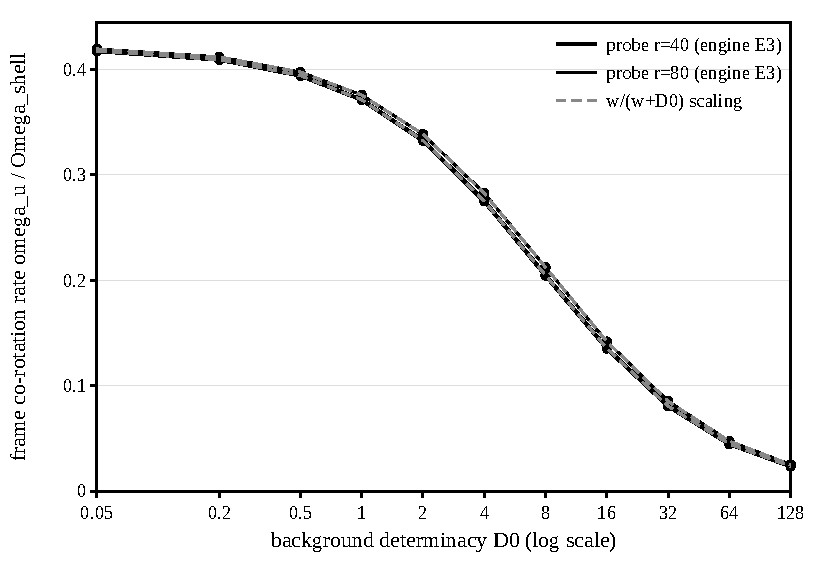
\includegraphics[width=\columnwidth]{fig1.pdf}
\caption{\label{fig:mach}%
Co-rotation rate of the local inertial frame,
$\omega_u/\Omega_{\rm shell}$, measured at interior probe points
($r = 40, 80$; four azimuths each) versus background determinacy
$\Dz$ (log scale), with the weight-fraction scaling
$\bar w/(\bar w+\Dz)$ (dashed).
Generated by \texttt{tools/gen-figures.mjs} from preset \texttt{mach}
(ring sources only, $\Omega_{\rm shell}=0.012$) with
$\Dz \in \{0.05,\dots,128\}$, reading the engine frame arrays (rule
E3); measured curve and scaling agree to $<0.1\%$.}
\end{figure}

\subsection{Experiment 2: outer-velocity enhancement from amplified
dragging}
\label{sec:exp2}

A disk system (central mass plus $n = 140$ disk particles) is run twice
from \emph{identical} initial conditions with $k_F = 1$ and $k_F = 0$
(the built-in Newtonian control, Sec.~\ref{sec:newton}).
With $k_F = 1$ the collective rotation feeds the frame field
$u_\varphi(r)$ and the outer stars are advected by the rotating frame,
raising the outer $v(r)$; with $k_F = 0$ the curve declines in
Keplerian fashion.
The machine gate (check V11) measures the outer-band
($r \in [85,130]$) mean tangential velocity difference, time-averaged
over steps 1000--2000: gain $0.055 \pm 0.007$ with control drift
$0.012$; the long-run CI variant measures an outer-band ratio
$v_{\varphi}(k_F{=}1)/v_{\varphi}(k_F{=}0) = 1.082$ at 6000 steps.
We deliberately gate this claim on the velocity \emph{enhancement},
not on flatness: a mean velocity difference does not measure the slope
of the curve, and a direct estimate of the outer logarithmic slope
$\beta = \ud\ln v_\varphi/\ud\ln r$ for this $N = 140$ disk is
noise-dominated (binned least-squares fits over the outer band give
$\beta \approx -0.2$ to $-0.5$ depending on band, binning, and epoch,
against $-0.5$ Keplerian; a single-epoch snapshot at 6000 steps gives
$\beta = -0.24$ versus $-0.47$ for the control).
The honest machine-gated statement is therefore a \emph{modest
outer-velocity enhancement} with a slope shallower than, or comparable
to, the Keplerian slope---not a demonstrated flat segment.
The self-consistent frame analysis further yields a
\emph{background-crossover scale}, $r_{\rm bg} \sim M_d/\Dz$, beyond
which the background determinacy screens the disk's frame contribution
and any enhancement must die away ($u_\varphi \to 0$, Keplerian
recovery); measuring the break radius by a $\Dz$ scan is left as an
optional exercise rather than claimed as a verified prediction.
This experiment is a demonstration of the mechanism within the model;
see negative claim~2.

\begin{figure}[t]
\centering
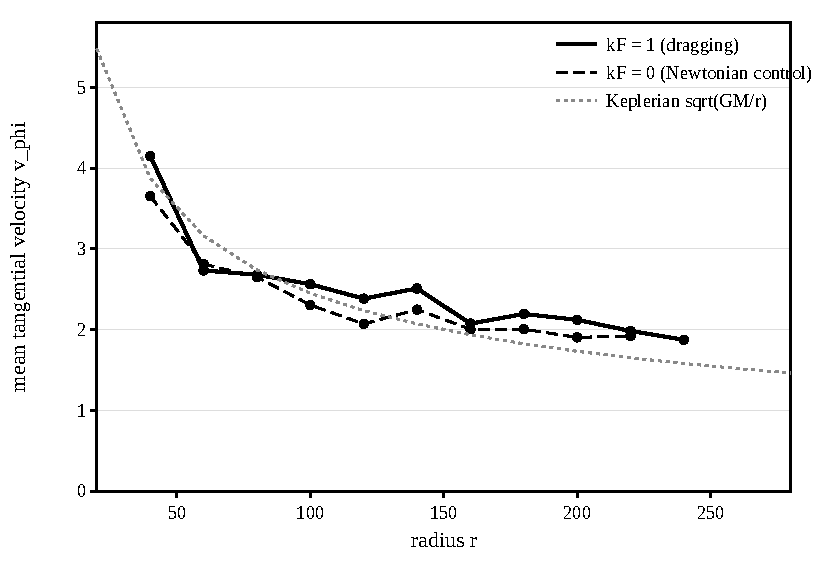
\includegraphics[width=\columnwidth]{fig2.pdf}
\caption{\label{fig:galaxy}%
Rotation curve $v_\varphi(r)$ for identical initial conditions with
$k_F = 1$ (enhanced outer velocities) and $k_F = 0$ (Keplerian
control), with the Keplerian expectation overlaid.
Generated from preset \texttt{galaxy} (central $m{=}600$, disk
$n{=}140$, $r{\le}130$, near-Keplerian initialization
$\times1.05$, $\Dz{=}0.5$) in the built-in A/B comparison mode;
quantitative gate: verification routine V11 (time-averaged outer-band
gain $0.055\pm0.007$).}
\end{figure}

\subsection{Experiment 3: periapsis regression and its reversal}
\label{sec:exp3}

An eccentric test orbit ($a = 60$, $e = 0.5$) around a pinned spinning
center is integrated with $k_F \in \{0,1\}$ and center spin
$S = \pm0.05$.
The automated check V6 measures $-7.52^\circ$/orbit (prograde spin:
regression), $+10.71^\circ$/orbit (spin reversed: advance), and
$-1.03^\circ$/orbit for the $k_F = 0$ numerical control---the sign
reverses under spin reversal, and the gate requires the effect to
exceed three times the numerical-control drift (the measured prograde
effect is about seven times the control).
A larger manual configuration ($a=120$, $e=0.5$, $S=+0.01$) gives
$-2.445^\circ$/orbit with near-linear scaling in $S$, and the
continuum-limit formula Eq.~(\ref{eq:prec}) reproduces sign, spin
scaling, and order of magnitude (measured coefficient
$c_p \approx 0.33$ relative to the far-field kernel approximation).
The interactive preset \texttt{drag} shows the same physics as a
rosette traced by the orbit trail ($-11.3^\circ$/orbit at its
parameters).

\begin{figure}[t]
\centering
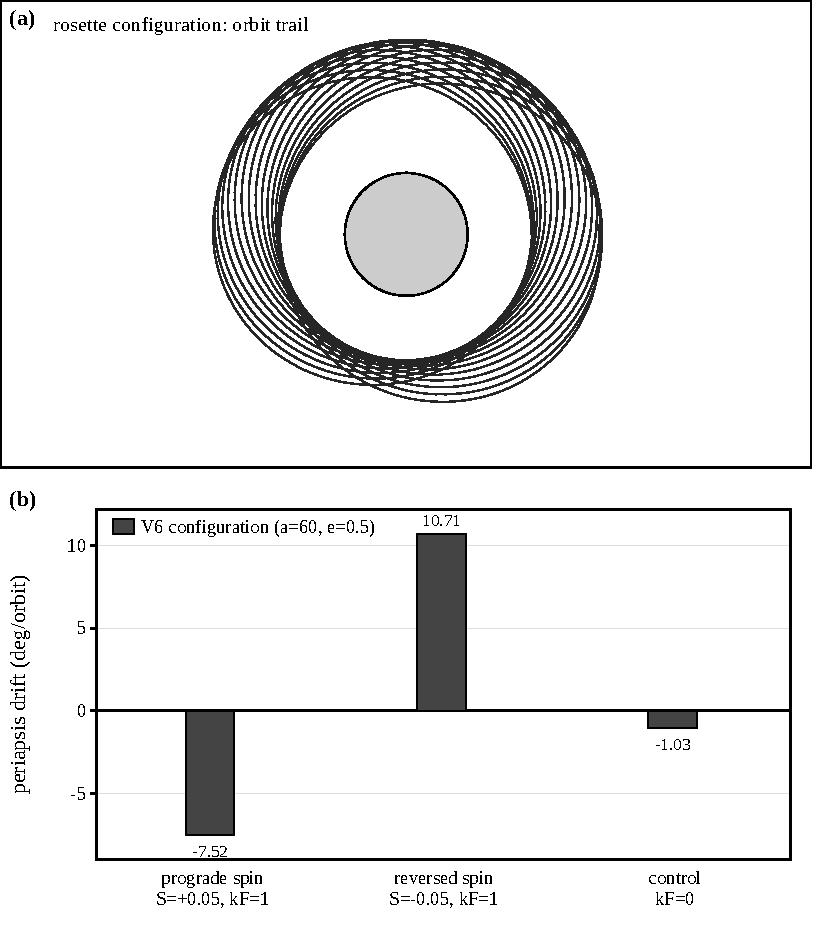
\includegraphics[width=\columnwidth]{fig3.pdf}
\caption{\label{fig:drag}%
(a)~Orbit trail over $\sim$8 orbits in preset \texttt{drag}: the
ellipse precesses opposite to the orbital motion (regression),
tracing a rosette.
(b)~Periapsis drift per orbit versus center spin sign:
regression $-7.52^\circ$ for prograde spin, advance $+10.71^\circ$
for reversed spin, control $-1.03^\circ$ at $k_F{=}0$.
Generated by \texttt{tools/gen-figures.mjs} from the V6 configuration
($a{=}60$, $e{=}0.5$, $S{=}\pm0.05$, $k_F\in\{0,1\}$, $\Dz{=}0.05$,
dissipation off; periapsis detection with $r$-gate and minimum
spacing) and preset \texttt{drag} (168\,000 steps).}
\end{figure}

\subsection{Experiment 4: clocks---gravitational plus kinematic, and
the twins}
\label{sec:exp4}

Three machine checks exercise E7R against analytic values:
(i) pure kinematic dilation (V12): with the gravitational term
suppressed, $\tau/t = 1.0000/0.9540/0.8001$ at $v/c_0 = 0, 0.3, 0.6$
versus theory $1/0.9539/0.8000$ (max relative error
$9.1\times10^{-5}$);
(ii) combined gravitational $+$ kinematic dilation on a circular orbit
(V13): $\tau/t = 0.8629$ versus the analytic value (relative error
$6.8\times10^{-6}$); this check doubles as a self-field-exclusion
detector;
(iii) the twin configuration (V16): a circling clock at $v = 0.5c_0$
against a reference clock at rest in the local frame,
$\tau_B/t = 0.8174$,
$\tau_A/t = 0.9672$, both matching the analytic integrals, with no
discontinuity in any clock at turnaround (step-to-step variation
$4.8\times10^{-7}$).
In DFM's preferred-frame representation the twin outcome is a plain
worldline integral of Eq.~(\ref{eq:A7}); the conceptual apparatus
associated with the ``paradox'' of relative simultaneity never enters.
We emphasize the delimitation recorded in the model documents: this is
a simplification of \emph{representation}, not a refutation of
relativity---standard relativity also resolves the twins uniquely by
proper-time integration.
The interactive preset \texttt{twin} displays three clocks with
$\tau/t = 1.000/0.874/0.611$.

\begin{figure}[t]
\centering
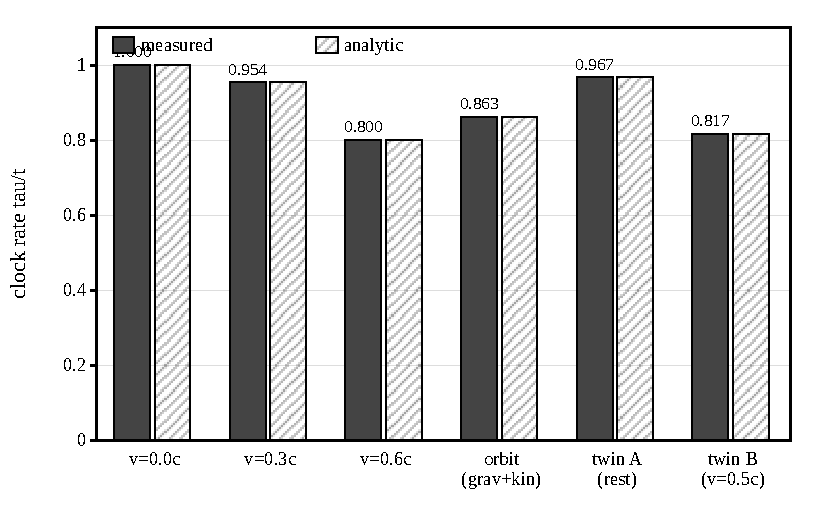
\includegraphics[width=\columnwidth]{fig4.pdf}
\caption{\label{fig:clocks}%
Measured and analytic clock rates $\tau/t$ for the kinematic
(V12), combined gravitational$+$kinematic (V13), and twin (V16)
configurations; the worst relative deviation across all six clocks is
$9.1\times10^{-5}$.
Generated by \texttt{tools/gen-figures.mjs} from the V12/V13/V16
configurations at their embedded parameters (V12: $\Kt{=}10^6$,
$v/c_0\in\{0,0.3,0.6\}$; V16: $v{=}0.5c_0$), 1000 steps each;
interactive counterpart: preset \texttt{twin}.}
\end{figure}

\subsection{Experiment 5: light---deflection, capture, and asymmetric
bending}
\label{sec:exp5}

A fan of 26 parallel rays is traced through the field of a compact
mass (preset \texttt{lensing}, $\Kt = 150$): mean bending angle
$48.6^\circ$, with five rays captured into circulating paths that
persist for the duration of the integration---an optical analogue of a
photon sphere (no claim of black-hole or event-horizon physics is
made).
With a spinning center (preset \texttt{spinlens}), the two sides of
the ray fan bend unequally---the medium advection term
$\vect{u}$ in Eq.~(\ref{eq:E8}) speeds prograde rays and retards
retrograde ones (a Kerr-like optical asymmetry, T8).
The machine gate V8 (run at $\Kt = 500$ for coefficient sensitivity)
measures the asymmetry at $6.77\times10^{-2}$~rad, proportional to the
center spin.

\begin{figure}[t]
\centering
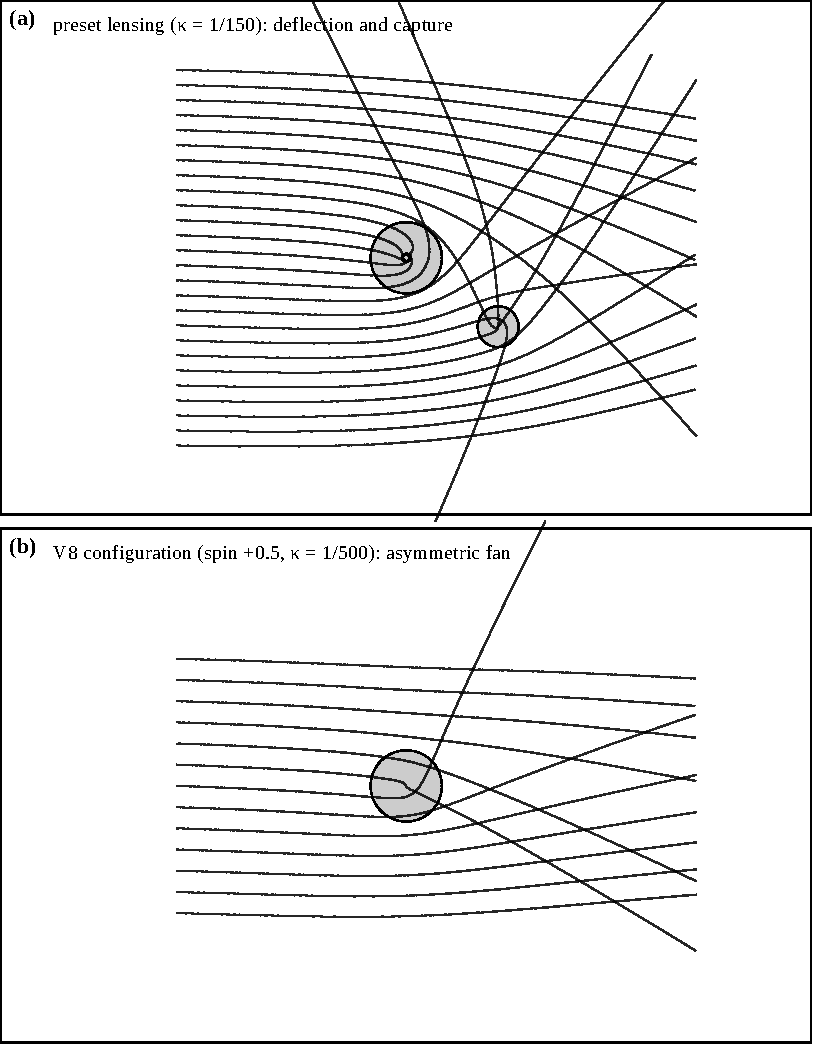
\includegraphics[width=\columnwidth]{fig5.pdf}
\caption{\label{fig:light}%
(a)~Ray fan in preset \texttt{lensing} ($\Kt{=}150$, 26 rays,
$x_0{=}-300$, $|y_0|\le255$, $\ud l{=}2.73$): deflection toward the
masses and captured circulating rays (an optical analogue of a photon
sphere).
(b)~Ray fan in the V8 configuration (central mass 1500, spin $+0.5$,
$\Kt{=}500$): the upper and lower halves bend unequally because the
medium is advected by the rotating frame.
Generated by \texttt{tools/gen-figures.mjs} via the shared ray tracer
(rule E8R); quantitative gate: verification routine V8, asymmetry
$\pm6.77\times10^{-2}$~rad with sign reversing under spin reversal.}
\end{figure}

\subsection{Experiment 6: spin-as-heat---equilibration and pressure}
\label{sec:exp6}

Two demonstrations, both restricted to a single particle size, for
which spin uniformity and temperature uniformity coincide (L9):
(i) a hot/cold split gas (preset \texttt{gas}) equilibrates its
left/right mean temperatures through contact friction and spin
diffusion---the zeroth-law analogue T6;
(ii) a hot core inside a cold shell (preset \texttt{pressure})
expands, the spin repulsion of the heated particles pushing the shell
outward (mean core radius $34.5 \to 140.9$, a $4.1\times$ expansion
with a mild overshoot before settling)---pressure emerges from A10
without an explicitly imposed pressure law.
Because the \texttt{gas} run is dissipative (its booked channels cool
the whole system while the gap closes), we separate equilibration from
cooling with an \emph{isolated control} in the CI suite: with all
cooling and contact channels off
($\eta_{\rm rad} = \gamma_n = \mu_f = 0$; spin diffusion E10$'$ only)
a static hot/cold lattice closes its temperature gap exponentially at
a measured rate $1.8\times10^{-3}$ per unit time while total spin
angular momentum $\sum_i I_i s_i$ is conserved to the rounding floor,
and a two-body version of the same run reproduces the analytic
relaxation rate $\kappa_s\,g(d)$ of Eq.~(\ref{eq:E10}) to
$3\times10^{-5}$ relative error.
Equilibration is thus a property of the diffusion rule itself, not an
artifact of everything decaying to zero.
The spectral thermometer (check V2) provides an independent
consistency check linking A9 and A12$'$: spin inferred from radiated
color reproduces the true spin within $5\%$.
We repeat the delimitation of negative claim~6: these are qualitative
analogies; the model's equation of state scales as $\rho^2 T$ rather
than the ideal-gas $\rho T$ (L15), and no quantitative thermodynamic
claims are made.
The reason for the single-size restriction is that with unequal
particle sizes E10$'$ equalizes the angular velocity $s$, not the
temperature $T = I s^2$, so equipartition is broken and heat can flow
from a colder small particle to a hotter large one---which is why all
quantitative heat demonstrations here use one particle size (L9).

\begin{figure}[t]
\centering
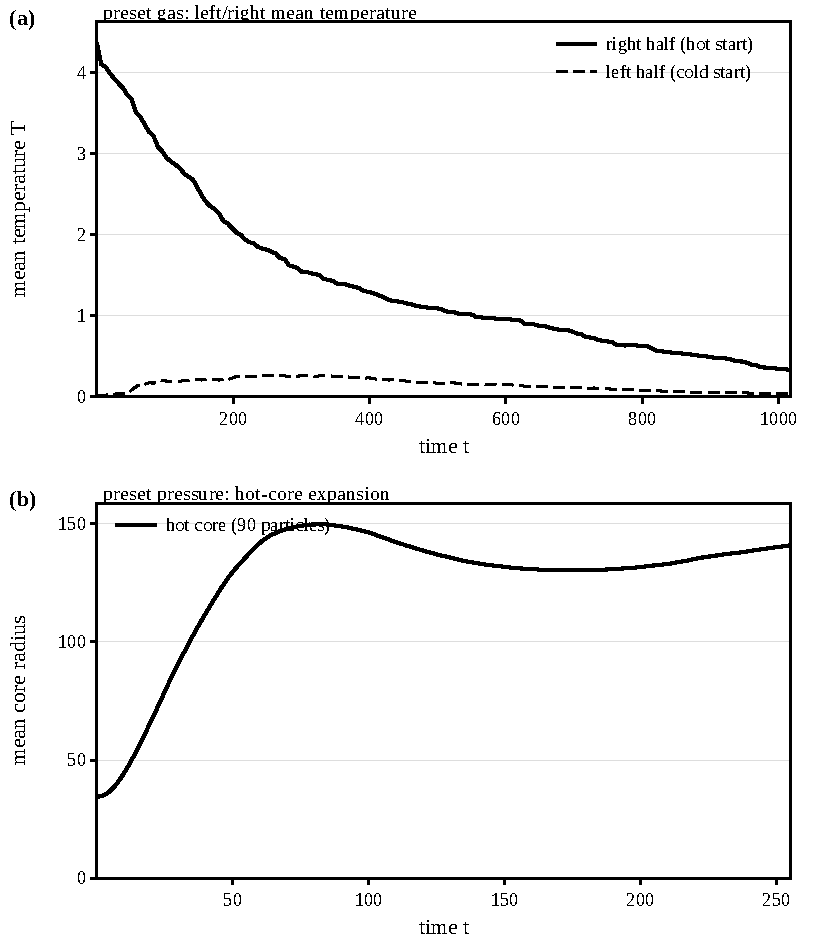
\includegraphics[width=\columnwidth]{fig6.pdf}
\caption{\label{fig:heat}%
(a)~Left/right mean temperature time series in preset \texttt{gas}
(single particle size): the initial gap of $4.3$ closes to $0.48$
while the total heat decays through the booked dissipation channels
(A12$'$)---equalization toward a common, slowly cooling temperature.
(b)~Hot-core expansion against a cold shell in preset
\texttt{pressure}: mean core radius $34.5 \to 140.9$.
Generated by \texttt{tools/gen-figures.mjs} from the named presets at
default parameters (16\,000 steps each) via \texttt{HP.sim}.}
\end{figure}

% =====================================================================
\section{Limitations and negative claims}
\label{sec:negative}

The following six statements are part of the paper's thesis, not
disclaimers appended to it.
Open problems referenced as L$n$ are cataloged in the project's
derivations document (Sec.~\ref{sec:repro}).

\subsection{Negative claim 1: not a description of the real universe}
DFM is not proposed as a description of nature.
It is a \emph{theory experiment}: the study of the consequences of a
counterfactual axiom system---``what if space were purely relational
and dragging were strong?''

\subsection{Negative claim 2: no statement about dark matter}
The outer-velocity-enhancement demonstration (experiment~2) does not
imply that dark matter is unnecessary.
In the real universe, GR frame dragging is suppressed by $v/c^2$ and is
orders of magnitude too weak, and the observational evidence bearing on
dark matter (CMB anisotropies, gravitational-lensing statistics,
structure formation) is independent and
strong~\cite{Planck2018}.
Experiment~2 demonstrates mechanism sufficiency \emph{within the
model}, nothing more.

\subsection{Negative claim 3: no Lorentz invariance, no causal
propagation}
The frame $\vect{u}$ and field $W$ are set instantaneously by the
global configuration (L8), and matter has no Lorentzian response
(L12): one-way light-speed isotropy for moving apparatus is not
reproduced.
Consequently the model cannot, in principle, describe binary-pulsar
orbital decay by gravitational radiation.

\subsection{Negative claim 4: two-dimensional only}
The model is 2D; no 3D quantitative predictions are made.
Spin is a scalar; a 3D extension (vector spin, vector dragging field,
angular-momentum alignment) is future work (L7).

\subsection{Negative claim 5: Mercury's perihelion advance is not
reproduced}
The observed main term ($+42.98''$/century) is a static 1PN effect.
DFM's static sector is exactly Newtonian
(Sec.~\ref{sec:newton}), and its dragging term E6$'$ yields only a
Lense--Thirring-sign \emph{regression} with a different radial power
[Eq.~(\ref{eq:prec})]; no single $k_F$ fits several planets at once
(a forced fit to Mercury mispredicts Venus by $1.38\times$, Earth by
$1.63\times$, Mars by $2.00\times$).
Meanwhile the clock-and-light sector does show formula-level benchmark
agreement at $\Kt = c^2/G$ (Table~\ref{tab:calib})---the model is
explicit about which sector works and which does not.

\subsection{Negative claim 6: thermodynamics is an analogy}
The heat sector is ``a 2D dissipative particle system with angular
momentum, given a temperature proxy $T = Is^2$ and a non-local
repulsion.''
It does not reproduce the ideal-gas equation of state (its spin
pressure scales as $\rho^2T$, and at the default $q = 2$ the 2D virial
integral diverges logarithmically with box size; L15), does not
contain latent heat or a phase variable (the solid/liquid/gas demo is
a morphological analogy; the model makes no claim of a
latent-heat phase transition), does not establish
Rayleigh--B\'enard criticality (no claim about the critical-Rayleigh
scaling law is made), and lacks detailed balance (it is a
dissipative granular-type system, not molecular dynamics converging to
canonical equilibrium; L16, L17), and breaks equipartition across
particle sizes (E10$'$ equalizes angular velocity, not $T = Is^2$,
so cold-to-hot heat flow between unequal sizes is possible; L9).
What does hold qualitatively, and only for a single particle size, is
the following: temperature equilibration, emergent pressure, and
conduction-like transport.

\subsection{Open problems}
\label{sec:limits}

The catalogue most relevant to this paper:
{\bf L1} (no action principle: E6$'$ is an update rule, not derived
from a Lagrangian---the leading open problem, see
Sec.~\ref{sec:conclusion});
{\bf L8} (instantaneous action at a distance);
{\bf L12} (no Lorentzian matter response);
{\bf L14} (cosmological $\Dz$ scale problem: counting all matter gives
$\Dz \sim 10^{27}\,{\rm kg\,m^{-1}} \approx \Kt$, whereas rotation
curves want $\sim10^{20}$---a seven-order-of-magnitude tension whose
resolution requires specifying which matter counts, linked to L8);
{\bf L15--L17} (thermodynamic sector: non-ideal equation of state and
its $q$-dependence; long-range conduction kernel; the spin-repulsion
potential bookkeeping that bounds the first-law claim domain).

% =====================================================================
\section{Conclusion and future work}
\label{sec:conclusion}

DFM shows how far a deliberately minimal, deliberately counterfactual
axiom system can go: one scalar field and one spin degree of freedom
mimic inertia, gravity, dragging, time dilation, light bending, and
thermodynamic behavior in a single running implementation, with the
conservation laws satisfied exactly at the equation level and every
principal numerical result verified by automated checks.
Its pedagogical value lies precisely in the pairing of a working
weak-field sector (Table~\ref{tab:calib}) with clearly delimited
failures (Sec.~\ref{sec:negative}): students can see \emph{both} in
the same tool, with the Newtonian control obtained by changing a
single parameter.

Three directions for future work are identified:

\paragraph*{(i) Action principle and geodesics (v2.0 core).}
The clock rule E7R defines a line element
\begin{equation}
c^2\ud\tau^2 = e^{-2\psi}c^2\ud t^2
 - e^{+2\psi}\left|\ud\vect{r}-\vect{u}\,\ud t\right|^2 ,
\label{eq:line}
\end{equation}
and the natural next step is to posit the particle action
$S = -mc^2\!\int\!\ud\tau$ and derive matter, clocks, and light from
one variational principle.
The static weak-field expansion of Eq.~(\ref{eq:line}) \emph{suggests}
PPN $\beta = \gamma = 1$---we state this strictly as a hypothesis to
be verified, since the field equations, the $\vect{u}\ne0$ geodesics,
and self-field exclusion remain undefined; if the program succeeds,
the static 1PN perihelion advance would arise naturally and $k_F$
would become a rotation-only parameter.
The branch criterion is fixed in advance: if the current E4/E6$'$
dynamics emerges as the slow-motion limit of the geodesics, v1 is
continuous with v2; if not, v1 is frozen as a phenomenological toy
and v2 is a different model.

\paragraph*{(ii) The $\Dz$ scale problem.}
Analyze a background/perturbation split $W = W_{\rm bg}(t) + \delta W$
first, then a causal field with a finite propagation speed, to address
the seven-order tension of L14.

\paragraph*{(iii) Quantitative thermodynamics profile.}
A separate parameter profile ($q = 3$, finite-range conduction,
periodic boundaries) for equation-of-state scans, decoupled from the
astrophysical demonstrations.

\section*{Reproducibility and companion tool}
\label{sec:repro}

The complete model---engine, twenty-five presets, verification suite,
and documentation (axioms, derivations, and the adjudication records
of all external AI review rounds)---is a single HTML file with no
external dependencies, archived with the project repository.
Code is released under the MIT license and documentation under
CC~BY~4.0, at \url{https://github.com/tty-imamura/dfm-simulator}.
The version of record for this paper will be fixed by a git tag on the
repository (\texttt{v1.23} series); the submission tag and a Zenodo
archival DOI minted from it will be inserted here at submission, so
that every number in the paper is tied to one immutable commit.
% TODO(submission): insert submission tag + Zenodo DOI here once minted.
Machine-verification outputs are part of that record: the
continuous-integration suite (\texttt{tests/qa.mjs}, 107 items
including the embedded \texttt{HP.verify.all()} checks, the time-step
sweep of Table~\ref{tab:verify}, and the isolated zeroth-law control
of Sec.~\ref{sec:exp6}) writes a machine-readable results file
(\texttt{tests/out/qa-results.json}, stamped with the git commit) that
is archived as supplementary material together with the per-figure
JSON records described below; the exact configurations (all physical
parameters, seeds, and step counts) of the verification runs quoted in
this paper are listed in Appendix~\ref{app:inputs}.
All figures in this paper are regenerated from the simulation by the
script \texttt{tools/gen-figures.mjs} (part of the repository), which
runs the presets and verification routines stated in each caption and
emits, next to each figure, a JSON record of the generation parameters
and measured values.
The companion tool also includes a weak-field calibration preset
(\texttt{grcal}) that displays the numbers of Table~\ref{tab:calib}
alongside their in-model analogue: a ground clock and an orbiting
satellite clock whose rates ($\tau/t = 0.920$ versus $0.971$)
reproduce the sign structure of the GPS offset---gravity beating
motion---with a ray fan showing the accompanying refraction.

\begin{acknowledgments}
Mathematical formalization, implementation, and verification were
carried out in collaboration with AI systems (Anthropic Claude);
external AI reviews (ChatGPT, Grok, Gemini) were used as adversarial
checks. All axioms and final decisions are the author's.
\end{acknowledgments}

% =====================================================================
\appendix

\section{SI restoration}
\label{app:si}

The simulator is dimensionless with $G = 1$.
For the ideal ($\varepsilon \to 0$) formulas:

\begin{table}[h]
\caption{\label{tab:si}SI restoration of the weak-field mapping.}
\begin{ruledtabular}
\begin{tabular}{llp{0.26\columnwidth}}
Quantity & Value & Note \\
\hline
$[W]$ & ${\rm kg\,m^{-1}}$ & determinacy dimension \\
$\Kt = c^2/G$ & $\approx 1.35\times10^{27}\ {\rm kg\,m^{-1}}$ &
clock/light coefficient \\
$2/\Kt = 2G/c^2$ & $\approx 1.48\times10^{-27}\ {\rm m\,kg^{-1}}$ &
effective lensing coefficient \\
\end{tabular}
\end{ruledtabular}
\end{table}

The effective lensing coefficient $2/\Kt$ is a derived combination
(Sec.~\ref{sec:dynamics}, E8R), not an independent parameter of the
model.
The softening $\varepsilon$ has no SI counterpart: it is numerical
regularization only.

A physical intuition for why the calibration constant is a \emph{line
density} (kg\,m$^{-1}$): the determinacy $W = \sum m/d$ itself has
mass-per-length dimension, and $\psi = W/\Kt$ reaches order unity
exactly when $GM/(c^2 d) \sim 1$, i.e.\ at the mass-to-radius ratio of
a relativistically compact system.
The same combination recurs as the mass-per-radius scale of the
observable universe ($GM_u/(c^2R_H) \sim 1$, the Sciama coincidence)
and in the ``maximum force'' $c^4/4G = \tfrac14(c^2/G)\,c^2$ discussed
in the GR literature.

% =====================================================================
\section{Benchmark inputs and verification configurations}
\label{app:inputs}

Table~\ref{tab:inputs} fixes every input behind the weak-field
benchmark rows of Table~\ref{tab:calib}; with these values and
$\Kt = c^2/G$, each number in that table is recomputable with no
further choices.
Two conventions apply to all rows: the model light speed is
$c_0 = c$, and the solar-system configuration is taken at rest in the
frame field ($\vect{u} = 0$; the DFM velocity in Eq.~(\ref{eq:A7}) is
then the ordinary orbital velocity).
Proper-time rates always exclude the clock's own field
($W_{\rm ext}$, A7$'$).

\begin{table}[h]
\caption{\label{tab:inputs}%
Observational inputs of the benchmark rows (Table~\ref{tab:calib}).}
\begin{ruledtabular}
\begin{tabular}{llp{0.30\columnwidth}}
Input & Value & Used in \\
\hline
$M_\oplus$ & $5.972\times10^{24}$ kg & GPS \\
$R_\oplus$ (ground clock) & $6.371\times10^{6}$ m & GPS \\
$r_{\rm GPS}$ (orbit radius) & $2.6562\times10^{7}$ m & GPS \\
$v_{\rm sat} = \sqrt{GM_\oplus/r_{\rm GPS}}$ & $3.87$ km/s & GPS \\
$v_{\rm ground} = \Omega_\oplus R_\oplus$ & $0.465$ km/s & GPS \\
$M_\odot$ & $1.989\times10^{30}$ kg & deflection, Shapiro \\
$R_\odot$ ($=b$) & $6.96\times10^{8}$ m & deflection, Shapiro \\
$r_1$ (Earth) & $1\ {\rm AU} = 1.496\times10^{11}$ m & Shapiro \\
$r_2$ (Saturn) & $8.43\ {\rm AU} = 1.261\times10^{12}$ m & Shapiro \\
geometry & superior conjunction, round trip & Shapiro \\
\end{tabular}
\end{ruledtabular}
\end{table}

Table~\ref{tab:vconfig} fixes the configurations of the verification
runs quoted in the text.
All runs are deterministic: random bodies are generated from a seeded
generator whose seed is derived from the stated preset ID, so
identical IDs reproduce identical initial conditions (a CI check
enforces this).
Parameters not listed take the engine defaults; the integrator step is
$\ud t = 0.016$ except in the V1 sweep.

\begin{table}[h]
\caption{\label{tab:vconfig}%
Verification-run configurations (embedded suite; preset IDs
\texttt{verify\_v1} etc.\ seed the deterministic layout generator).}
\begin{ruledtabular}
\begin{tabular}{lp{0.72\columnwidth}}
Run & Configuration \\
\hline
V1 & $\Dz{=}0$, $k_F{=}1$, $G{=}1$, $k_{\rm rep}{=}1$,
$\mu_f{=}0.5$, $\gamma_n{=}0.4$, $\kappa_s{=}0.05$,
$\eta_{\rm rad}{=}0$, $\varepsilon{=}2$; central $m{=}30$
($s{=}0.5$) $+$ disk $n{=}48$, $r{\le}120$, $m\in[0.5,2]$,
$s\in[-2,2]$, random velocities ($\times1.2$); 1000 steps
(sweep: $\ud t \in \{0.016,0.008,0.004\}$ at fixed $T{=}16$) \\
V9 & $G{=}1$, $\Dz{=}2$, $\varepsilon{=}2$; pinned $m{=}50$ at
origin, $m{=}20$ at $(18,-7)$, probe $m{=}0.01$ at three points;
central difference $h{=}0.01$ \\
V10 & $G{=}1$, $\Dz{=}0$, $k_F{=}0$, $k_{\rm rep}{=}0$,
$\mu_f{=}0.5$, $\gamma_n{=}0.4$, $\kappa_s{=}0.3$,
$\eta_{\rm rad}{=}2\times10^{-4}$ ($p{=}1$), $\varepsilon{=}2$;
37 particles (central $m{=}30$, $s{=}0.8$ $+$ disk $n{=}36$,
$r{\le}55$, $m\in[1,2]$, $s\in[-1.5,1.5]$); 1000 steps \\
V10b & $G{=}0$, $k_{\rm rep}{=}2$, all dissipation off; three
particles $m{=}2,3,2.5$ at stated positions with spins
$2,-1.5,1$; 1000 steps \\
V11 & $G{=}1$, $\Dz{=}0.5$, $\mu_f{=}0.02$, $\gamma_n{=}0.05$,
$k_{\rm rep}{=}1$, $\kappa_s{=}0.05$, $\varepsilon{=}4$; central
$m{=}600$ ($s{=}0.05$) $+$ disk $n{=}140$, $r{\le}130$,
$m\in[0.5,1.2]$, near-Keplerian ($\times1.05$); A/B with
$k_F{=}1/0$ from identical initial conditions; outer band
$r\in[85,130]$, time-averaged over steps 1000--2000 \\
Zeroth-law control & $G{=}0$, $k_F{=}0$, $k_{\rm rep}{=}0$,
$\mu_f{=}\gamma_n{=}\eta_{\rm rad}{=}0$, $\kappa_s{=}0.3$;
$8\times6$ static lattice (spacing 40), $m{=}1$, spins $0.3$
(left) / $2.5$ (right), 4000 steps; two-body variant $m{=}2$,
$d{=}30$, spins $2/0$, 2500 steps \\
\end{tabular}
\end{ruledtabular}
\end{table}

% =====================================================================
\section{The consequences T1--T9}
\label{app:theorems}

Table~\ref{tab:theorems} lists the consequences referenced in the
text, each with its dependencies, its conditions of validity, and its
machine gate where one exists.
Entries whose validity has been established only for particular
initial conditions and parameter ranges are marked
\emph{conditional numerical propositions} (CNP); they are not
theorems.

\begin{table*}[t]
\caption{\label{tab:theorems}%
The consequences T1--T9: statement, dependencies, status, and machine
gate.
CNP $=$ conditional numerical proposition (holds in the verified
configurations; no generality claimed).}
\begin{ruledtabular}
\begin{tabular}{lp{0.34\textwidth}p{0.13\textwidth}p{0.14\textwidth}p{0.17\textwidth}}
ID & Statement & Depends on & Status & Machine gate \\
\hline
T1 & For $N{=}1$, $\Dz{=}0$: $\vect{u} \equiv \vect{v}_1$, so
single-particle translation and rotation are undetectable in
principle & A3, A4 & exact identity & (constructive; enters V12
frame handling) \\
T2 & Near a dominant mass, $\vect{u} \to \vect{v}_j$: space is
dragged along; for $\Dz \gg \sum w$, $\vect{u} \to 0$ & A3, A4 &
limit statement & experiment 1 scaling
$\bar w/(\bar w{+}\Dz)$, $<0.1\%$ \\
T3 & Contact friction circularizes orbits and aligns spins (2D) &
A9, E9 & CNP & preset demonstrations (\texttt{saturn}) \\
T4 & Collective disk rotation feeds $u_\varphi$; outer orbital
velocities are enhanced over the $k_F{=}0$ control
(outer-velocity enhancement; no flatness claim) & A5, E3, E6$'$ &
CNP & V11 (gain $0.055\pm0.007$); CI ratio 1.082 \\
T5 & Light bends toward mass with $n_{\rm eff} = e^{2\psi}$;
strong fields capture rays (optical photon-sphere analogue) &
A7$'$, A11, E8R & weak-field formula $+$ CNP & deflection formula
(Table~\ref{tab:calib}); capture in preset \texttt{lensing} \\
T6 & Spin-as-heat equilibrates temperature (zeroth-law analogue)
and generates pressure (valid only for a single particle size) & A9,
A10,
E5$'$, E9, E10$'$ & CNP (single size; L9) & \texttt{gas} /
\texttt{pressure} gates; isolated zeroth-law control
(Sec.~\ref{sec:exp6}) \\
T7 & With $\Dz{=}0$, no pinned particles: $\vect{P}$ and
$L_{\rm tot}$ exactly conserved; $\Dz{>}0$ deficits equal the
reservoir ledger & A13, E4, E5$'$, E6$'$, E9, E10$'$ &
equation-level theorem (proof in Sec.~\ref{sec:dynamics}) & V1
(residual at rounding floor, $\ud t$-independent) \\
T8 & A spinning center bends prograde and retrograde rays
unequally, asymmetry $\propto k_F u_\varphi$ (Kerr-like optical
analogue) & A8, A11, E8R & CNP & V8 (asymmetry
$6.77\times10^{-2}$ rad, sign reverses with spin) \\
T9 & Reunion clock differences are unique worldline integrals of
Eq.~(\ref{eq:A7}); ``mutual time dilation'' is a representation
effect of observer-centered synchronization (not a refutation of
relativity---a representation simplification) & A11, E7R &
representation statement & V16 (twin clocks match analytic
integrals; no discontinuity) \\
\end{tabular}
\end{ruledtabular}
\end{table*}

% =====================================================================
% Bibliography.  All entries verified against primary/near-primary
% records (publisher, NASA ADS, INSPIRE, WorldCat, arXiv) on
% 2026-07-18; cross-checked by three independent AI reviews.
\begin{thebibliography}{99}

\bibitem{Newton1687}
I.~Newton, \emph{Philosophi\ae{} Naturalis Principia Mathematica}
(Jussu Societatis Regi\ae{} ac Typis Josephi Streater, Londini, 1687),
Scholium to the Definitions.

\bibitem{Mach1883}
E.~Mach, \emph{Die Mechanik in ihrer Entwickelung:
historisch-kritisch dargestellt} (F.~A.~Brockhaus, Leipzig, 1883);
English trans.\ T.~J.~McCormack, \emph{The Science of Mechanics:
A Critical and Historical Exposition of Its Principles}
(Open Court Publishing Co., Chicago, 1893).

\bibitem{Sciama1953}
D.~W.~Sciama, ``On the origin of inertia,''
Mon.\ Not.\ R.\ Astron.\ Soc.\ \textbf{113}, 34--42 (1953),
\href{https://doi.org/10.1093/mnras/113.1.34}
{doi:10.1093/mnras/113.1.34}.

\bibitem{BarbourBertotti1982}
J.~B.~Barbour and B.~Bertotti, ``Mach's principle and the structure of
dynamical theories,''
Proc.\ R.\ Soc.\ Lond.\ A \textbf{382}, 295--306 (1982),
\href{https://doi.org/10.1098/rspa.1982.0102}
{doi:10.1098/rspa.1982.0102}.

\bibitem{LenseThirring1918}
J.~Lense and H.~Thirring, ``\"Uber den Einflu\ss{} der Eigenrotation
der Zentralk\"orper auf die Bewegung der Planeten und Monde nach der
Einsteinschen Gravitationstheorie,''
Phys.\ Z.\ \textbf{19}, 156--163 (1918),
ADS bibcode: 1918PhyZ...19..156L; English translation in
Gen.\ Relativ.\ Gravit.\ \textbf{16}, 727--741 (1984),
\href{https://doi.org/10.1007/BF00759853}{doi:10.1007/BF00759853}.

\bibitem{Everitt2011}
C.~W.~F.~Everitt \emph{et al.}, ``Gravity Probe B: Final results of a
space experiment to test general relativity,''
Phys.\ Rev.\ Lett.\ \textbf{106}, 221101 (2011),
\href{https://doi.org/10.1103/PhysRevLett.106.221101}
{doi:10.1103/PhysRevLett.106.221101}.

\bibitem{CiufoliniPavlis2004}
I.~Ciufolini and E.~C.~Pavlis, ``A confirmation of the general
relativistic prediction of the Lense--Thirring effect,''
Nature \textbf{431}, 958--960 (2004),
\href{https://doi.org/10.1038/nature03007}{doi:10.1038/nature03007}.

\bibitem{RubinFord1970}
V.~C.~Rubin and W.~K.~Ford, Jr., ``Rotation of the Andromeda nebula
from a spectroscopic survey of emission regions,''
Astrophys.\ J.\ \textbf{159}, 379--403 (1970),
\href{https://doi.org/10.1086/150317}{doi:10.1086/150317}.

\bibitem{Milgrom1983}
M.~Milgrom, ``A modification of the Newtonian dynamics as a possible
alternative to the hidden mass hypothesis,''
Astrophys.\ J.\ \textbf{270}, 365--370 (1983),
\href{https://doi.org/10.1086/161130}{doi:10.1086/161130}.

\bibitem{Planck2018}
Planck Collaboration, ``Planck 2018 results. VI. Cosmological
parameters,'' Astron.\ Astrophys.\ \textbf{641}, A6 (2020),
\href{https://doi.org/10.1051/0004-6361/201833910}
{doi:10.1051/0004-6361/201833910};
Erratum: Astron.\ Astrophys.\ \textbf{652}, C4 (2021),
\href{https://doi.org/10.1051/0004-6361/201833910e}
{doi:10.1051/0004-6361/201833910e}.

\bibitem{CooperstockTieu2005}
F.~I.~Cooperstock and S.~Tieu, ``General relativity resolves galactic
rotation without exotic dark matter,'' arXiv:astro-ph/0507619 (2005),
\href{https://arxiv.org/abs/astro-ph/0507619}
{arXiv:astro-ph/0507619}.

\bibitem{FuchsPhleps2006}
B.~Fuchs and S.~Phleps, ``Comment on `General relativity resolves
galactic rotation without exotic dark matter','' New Astron.\
\textbf{11}, 608--610 (2006),
\href{https://doi.org/10.1016/j.newast.2006.04.002}
{doi:10.1016/j.newast.2006.04.002}.

\bibitem{Korzynski2007}
M.~Korzy\'nski, ``Singular disk of matter in the Cooperstock--Tieu
galaxy model,'' J.\ Phys.\ A: Math.\ Theor.\ \textbf{40}, 7087--7092
(2007),
\href{https://doi.org/10.1088/1751-8113/40/25/S66}
{doi:10.1088/1751-8113/40/25/S66}.

\bibitem{Ludwig2021}
G.~O.~Ludwig, ``Galactic rotation curve and dark matter according to
gravitomagnetism,'' Eur.\ Phys.\ J.\ C \textbf{81}, 186 (2021),
\href{https://doi.org/10.1140/epjc/s10052-021-08967-3}
{doi:10.1140/epjc/s10052-021-08967-3}.

\bibitem{LasenbyHobsonBarker2023}
A.~Lasenby, M.~P.~Hobson, and W.~Barker, ``Gravitomagnetism and galaxy
rotation curves: a cautionary tale,'' Class.\ Quantum Grav.\
\textbf{40}, 215014 (2023),
\href{https://doi.org/10.1088/1361-6382/acef8b}
{doi:10.1088/1361-6382/acef8b}.

\bibitem{deFelice1971}
F.~de~Felice, ``On the gravitational field acting as an optical
medium,'' Gen.\ Relativ.\ Gravit.\ \textbf{2}, 347--357 (1971),
\href{https://doi.org/10.1007/BF00758153}{doi:10.1007/BF00758153}.

\bibitem{Unruh1981}
W.~G.~Unruh, ``Experimental black-hole evaporation?''
Phys.\ Rev.\ Lett.\ \textbf{46}, 1351--1353 (1981),
\href{https://doi.org/10.1103/PhysRevLett.46.1351}
{doi:10.1103/PhysRevLett.46.1351}.

\bibitem{BarceloLiberatiVisser2005}
C.~Barcel\'o, S.~Liberati, and M.~Visser, ``Analogue gravity,''
Living Rev.\ Relativity \textbf{8}, 12 (2005),
\href{https://doi.org/10.12942/lrr-2005-12}{doi:10.12942/lrr-2005-12}.

\bibitem{LyndenBellKatz1995}
D.~Lynden-Bell and J.~Katz, ``Classical mechanics without absolute
space,'' Phys.\ Rev.\ D \textbf{52}, 7322--7324 (1995),
\href{https://doi.org/10.1103/PhysRevD.52.7322}
{doi:10.1103/PhysRevD.52.7322}.

\bibitem{Assis1999}
A.~K.~T.~Assis, \emph{Relational Mechanics}
(Apeiron, Montreal, 1999).

\bibitem{Bertotti2003}
B.~Bertotti, L.~Iess, and P.~Tortora, ``A test of general relativity
using radio links with the Cassini spacecraft,''
Nature \textbf{425}, 374--376 (2003),
\href{https://doi.org/10.1038/nature01997}{doi:10.1038/nature01997}.

\bibitem{Verlinde2017}
E.~Verlinde, ``Emergent gravity and the dark universe,''
SciPost Phys.\ \textbf{2}, 016 (2017),
\href{https://doi.org/10.21468/SciPostPhys.2.3.016}
{doi:10.21468/SciPostPhys.2.3.016}.

\bibitem{BrilliantovPoschel2004}
N.~V.~Brilliantov and T.~P\"oschel,
\emph{Kinetic Theory of Granular Gases}
(Oxford University Press, Oxford, 2004),
\href{https://doi.org/10.1093/acprof:oso/9780198530381.001.0001}
{doi:10.1093/acprof:oso/9780198530381.001.0001}.

\bibitem{IorioMercury2011}
L.~Iorio, ``Mercury and frame-dragging in light of the MESSENGER
flybys: towards a new test of general relativity?''
arXiv:1109.0266 (2011),
\href{https://arxiv.org/abs/1109.0266}{arXiv:1109.0266}.

\bibitem{IorioEtAl2011}
L.~Iorio, H.~I.~M.~Lichtenegger, M.~L.~Ruggiero, and C.~Corda,
``Phenomenology of the Lense--Thirring effect in the Solar System,''
Astrophys.\ Space Sci.\ \textbf{331}, 351--395 (2011),
\href{https://doi.org/10.1007/s10509-010-0489-5}
{doi:10.1007/s10509-010-0489-5}.

\end{thebibliography}

\end{document}
